% !TEX root = ../thesis_main.tex
\chapter{Materials and methods}\label{chap:MaterialsAndMethods}
\label{chapter:matMeth}
    \section{Parahydrogen generation and quantification}
    Parahydrogen was generated using a coldhead surrounding a chamber of $\mathrm{FeO_4}$ catalyst which was built before the beginning of this work \cite{hovener_continuous-flow_2013}. The setup is positioned on top of the laboratory building's roof for safety reasons with the coldhead and the complete hydrogen system on the outside and the temperature sensitive equipment such as the vacuum pump or the helium recondenser on the inside. Holes were drilled to feed the connections for vacuum hoses, sensor cables and pump exhaust through the wall.
    \begin{figure}
        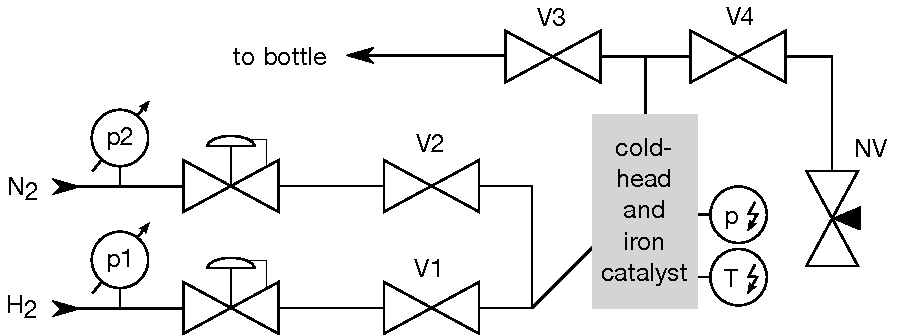
\includegraphics[width=0.99\textwidth]{/figures/materialsMethods/setupParahydrogenGenerator.pdf}
        \caption[Parahydrogen generator scheme]{The schematics of the parahydrogen generator's valve system used for reproducible and continuous production of pH2. In the lower left, the two gases, H$_2$ and N2 are inserted into the system at defined pressures. After flowing through the central part, the coldhead, the flow against ambient pressure can be set via the needle valve before redirecting it towards the bottle to be filled.}
        \label{figure:materialsMethods:pH2Generator}
    \end{figure}
        \subsection{Coldhead side}
            The coldhead was cooled down to \SI{21}{\kelvin} via a water-cooled helium recondenser with a closed helium circuit. The recondenser was operated at full power while a counteracting heater was used to keep temperatures at 21 K. The coldhead was isolated from surroundings by a vacuum chamber pumped down by a rotary vane pump. A pressure sensor was attached to the vacuum chamber to ensure sufficient isolation before switching on the helium recondenser. Temperature sensors in the catalyst chamber and on top of the coolant line were used for checking whether the conversion can be started and also as a feedback for the heater to regulate temperature.
        \subsection{Hydrogen side}
            The system was usually flooded with nitrogen gas before use to ensure that no explosive mixtures could build up. As the nitrogen freezing point is at \SI{63}{\kelvin}, it needed to be removed before cooling. This was achieved by flushing the system with neat hydrogen gas. The system consisted of the hydrogen and nitrogen supply bottles (both \SI{10}{\liter}, \SI{200}{\bar}, 99.999\% pure), both with individual pressure regulators and additional cutoff valves. The lines from the supply bottles then combine into a single line running towards and trough the coldhead and its catalyst chamber where the conversion occurs. Behind that coldhead, a needle valve regulates flow and can be switched between a flow meter to measure and set the flow against atmospheric pressure and a bottle storing the parahydrogen. Pressure limits given by the manufacturer are \SI{50}{\bar}. 
        \subsection{Parahydrogen quantification}
            To quantify the parahydrogen fraction of the gas bottled at the generator, NMR spectra of the gas were recorded. As pH$_2$ is NMR invisible, the signal drops with the increase in parahydrogen fraction. To record the spectra, the gas was filled into a laboratory glass tube that was thoroughly cleaned and put into a $^{1}$H quadrature coil for detection inside the MRI. It had to be ensured that the measured spectrum was compared to a nitrogen sample inside the same tube to subtract background signal from tube and plug. Additionally, a spectrum of thermal hydrogen was recorded off which the parahydrogen content is known. The parahydrogen fraction was calculated as follows:
            \begin{equation}
                \frac{S_{pH2}-S_{N2}}{S_{H2}-S_{N2}} = \frac{f_{pH2}}{\tfrac{3}{4}} = \frac{4}{3} \cdot xx \rightarrow f_{pH2} = \frac{4}{3} \frac{S_{pH2}-S_{N2}}{S_{H2}-S_{N2}}
            \end{equation}
            where $f_{pH2}$ is the parahydrogen fraction, $S_{pH2}$ is the signal of the pH$_2$ enriched gas, $S_{H_2}$ is the signal of thermal Hydrogen and $S_{N_2}$ is the background signal measured with nitrogen gas that is subtracted.
        \subsection{Parahydrogen decay}
            To monitor the lifetime of parahydrogen, the quantification method was used multiple times over the course of days. The decrease in parahydrogen fraction could be monitored and may be different for different means of storage, i.e. in our case, different bottles.
        \section{Low field Spectrometer}
        \label{sec:matMeth:lowFieldSpectrometer}
        To acquire NMR spectra at fields where 1H-Sabre is feasible \cite{rayner_signal_2018}, a low field NMR spectrometer was built \cite{borowiak_battery-driven_2013-1} previous to this work as shown in figure \ref{figure:materialsMethods:lowFieldSpec}. Its main field is generated by a resistive coil in solenoid or a newly developed dual Helmholtz assembly design \ref{sec:matMeth:Helmholtz}. Inside that coil, there is a saddle coil generating a $B_1$ field perpendicular to $B_0$. Inside and perpendicular to both, a third coil, usually a solenoid, is used to detect the signal generated through the spin manipulation. All coils were wound by hand, partly using dedicated molds to generate specific shapes. After winding the coils, they were fixed using dual component epoxy glue (UHU Plus "sofortfest", UHU GmbH).
        All coils are easily exchangeable, e.g. the B0 coil can be switched to another one if a more sophisticated design is desired or other requirements arise. Also, differently sized samples or different nuclei can be measured by exchanging the receive coil. The transmit coil is already wide band and thus can be used on a wider range of nuclei, but is also part of the modular setup. The B0 coil is connected via banana jacks using unshielded cables while the RF signal and NMR signal are routed via coaxial cable using BNC  and SMA plugs respectively.
        \begin{figure}
            \label{figure:matMeth:lowFieldSpectrometer}
            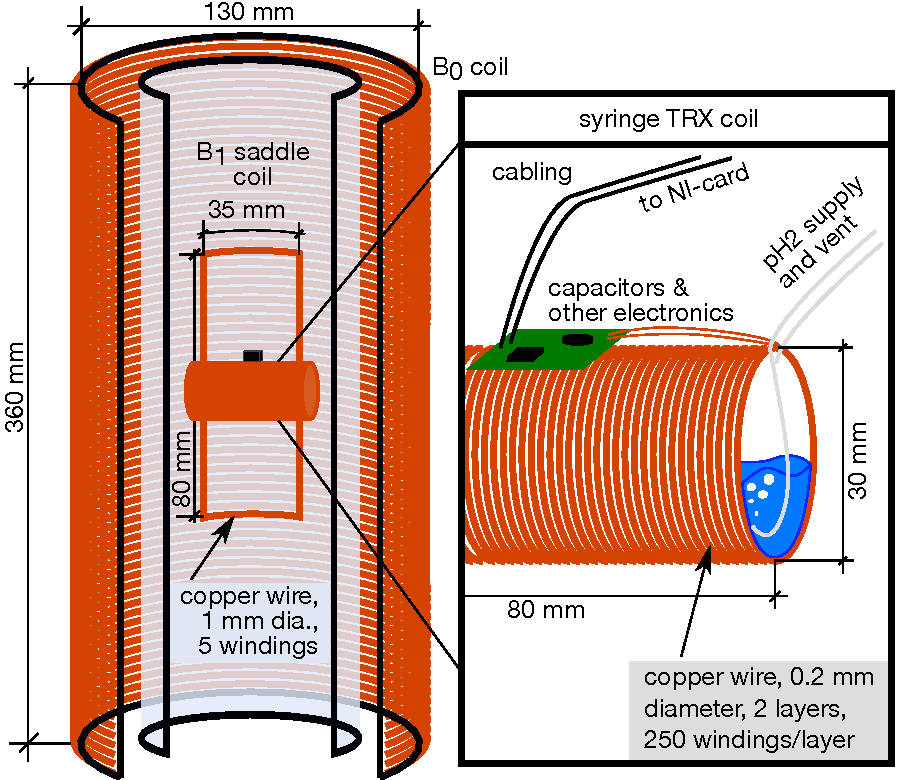
\includegraphics[width=0.99\textwidth]{/figures/materialsMethods/lowFieldSpectrometer/spectrometer.pdf}
            \caption[Schematic view low field spectrometer]{A cut view of the low field spectrometer used in the experiments. Note that only one of the two saddle coils is displayed, the other is exactly opposite of the first with the current flowing in the same chirality producing a magnetic field adding to that of the other coil in the ROI. }
            \label{figure:materialsMethods:lowFieldSpec}
        \end{figure}
        \subsection{Static magnetic field}
        Multiple coil designs of the static field generating coils have been  considered, simulated, built and tested in the course of this work. The previously used solenoid design with different lengths of compensation windings (section \ref{sec:simulations:B0sim}) showed to have disadvantages over the dual Helmholz assembly built during this work.
        \subsubsection{Solenoid coil}
            The $B_0$ coil is wound around an acrylic tube in two full layers. In addition, at the
            tube's ends, compensation windings are installed to homogenize the field inside the coil.
            The length of these windings was optimized in Matlab simulations (section \ref{sec:simulations:B0sim})
            Coils usually consist of one or more layers of wire usually wound around an acrylic tube. Spacing between layers is given by wire thickness including insulation coating. To keep  these distances small and, in turn, current- and thus magnetic flux density high, enameled wire was used for all coils. Winding of the wire was mostly performed on a turning lathe enabling automatic counting of the number of windings and a steady, consistent feed of the wire.
            The solenoid coil used in the main low field experiments consisted of a three layered solenoid with two layers of compensation windings on each side. \SI{1}{\mm} diameter enameled copper wire was used to build the B0 coil. The main layers consisted of 362 windings with an inner diameter of \SI{120}{\mm}. The overall length is \SI{350}{\milli\meter}. The length of the compensation windings was \SI{48}{\mm}.
            \begin{figure}
                \centering
                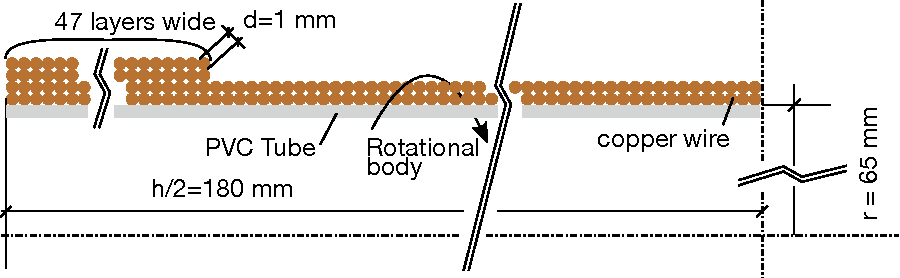
\includegraphics[width=0.99\textwidth]{/figures/materialsMethods/lowFieldSpectrometer/B0Solenoid.pdf}
                \caption[B0 coil layout]{Dimensions and structure of the standard B0 solenoid coil used in the low field experiments to generate a homogeneous field. Note the two additional layers of wiring (compensation windings) on the left homogenize the field to levels above the pure solenoid's homogeneity.}
                \label{fig:matMeth:b0Solenoid}
            \end{figure}
        \subsubsection{Helmholtz coil}
        \label{sec:matMeth:Helmholtz}
        As in the solenoid case, before building the dual Helmholtz array, simulations were performed.  As space was limited inside the Mu metal shield where the coil was supposed to be used in, the coils' diameters were predetermined and only their distances and currents were optimized (see sec. \ref{simulations:B0} for details). As for the general setup, an acrylic tube onto which four coil holders were mounted was chosen as a coil holder. Using the simulation results, a layout for the coil holders was designed. To keep unwanted fields due to connecting wires to a minimum, these wires were kept as short as possible. Holders were lathed and then processed further by hand. Winding of the wire was also done by hand. To keep the wire form sliding into the gouges of the previous layer, PVC foil was laser cut to fit the dimensions of the coil holders. Due to the limited size of the foil used (Din A4) and the relatively large diameter of the coils, three stripes of foil were connected with one of the three parts employing a feedthrough for the wire traversing from one layer to the next (see figure \ref{fig:appendix:helmholtzParts}).
        \subsection{Radiofrequency excitation}
        \label{sec:matMeth:rfPulses}
        The saddle coils are aligned in a way that they show axial symmetry around the rotational axis of the PVC tube they're mounted on. The dimensions were chosen to fit the ratio mentioned in the theory section (\ref{sec:theory:saddleCoils}), i.e. \SI{10}{\cm} by \SI{20}{\cm}, corresponding to an angle of $\approx$\SI{240}{\degree} covered by the coils (\SI{120}{\degree} per coil). The number of windings per coil was 6, wire leads to and from the coils were parallelized as far as possible to minimize additional field generation not covered in the simulations. 
        The initial coil shape was flat, which facilitated winding the coil inside a wire holder. The holder was a rectangular, two parted slitted aluminum plate. The wire was wound into the slit and formed a stacked design. Then the wire layers were glued together to construct a solid connection between them. After being removed from the holder, the assembly is bent into shape using a smaller diameter acrylic tube so that, after, the radius compares to that of the larger acrylic tube. The coil was operated untuned and unmatched as a broadband excitation coil. The pulse generation was performed using a National Instruments data acquisition crate (NI USB-6251, National Instruments) which's signal was amplified with an audio amplifier (TX-8555 Stereo Receiver, Onkyo).
            The pulse was constructed using the hypercontrol software described later (\ref{sec:matMeth:hypercontrol}). Generally, block pulses were used but arbitrary pulseforms are possible with the card as long as the contained frequencies are below \SI{500}{\kilo\hertz} (Nyquist-Shannon). 
            \begin{figure}
                \label{fig:matMeth:amplifierResponse}
                \centering
                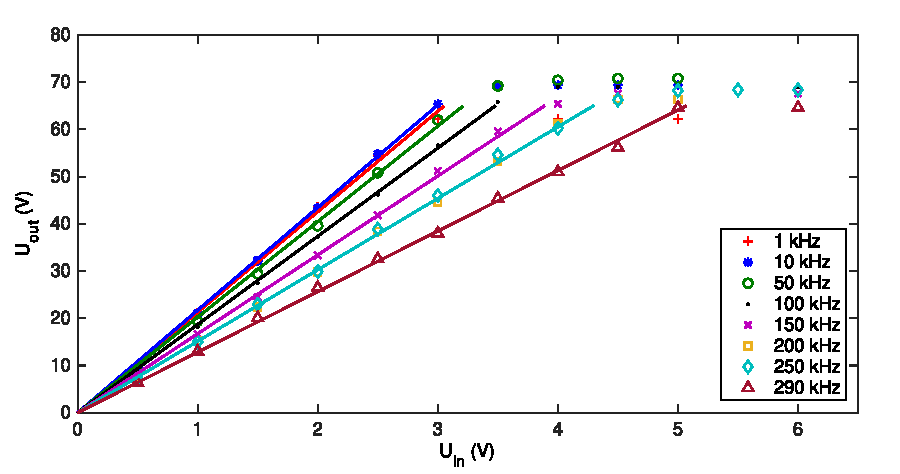
\includegraphics[width=0.99\textwidth]{/figures/materialsMethods/lowFieldSpectrometer/amplifierResponse.pdf}
            \caption[Amplifier response]{The response of the Onkyo audio amplifier at different frequencies as used in the low field spectrometer. Note the saturation at input voltages above 3 to 5 \si{\volt}. Also note that for higher frequencies, the amplification is lower, as the amplifier was designed for frequencies below \SI{150}{\kilo\hertz}. That is why, even at maximum amplification, only \SI{180}{\degree} flip angles were possible using pulselengths below \SI{1}{\milli\second}.}
            \end{figure}
        \subsection{Receive coil}
        \label{sec:matMeth:receiveCoil}
        For signal reception, multiple coils of different resonance frequencies were built for use at different fields and for different purposes. The two coils mostly used in the low field spectrometer were a larger diameter coil used in field homogeneity testing and for $^{13}$C experiments and a $^{1}$H coil wound around a syringe that also featured tubing for gas in- and outlet (mostly hydrogen) in hyperpolarization experiments. The diameter of the syringe, and thus the coils inner diameter was \SI{30}{\mm} with a length of \SI{56}{\milli\meter}. The total volume was \SI{39}{\milli\liter}. It consisted of two layers of \SI{0.3}{\milli\meter} copper wire wound around the syringe in close packing. The number of windings was 180 per layer. A \SI{0.47}{\micro\farad} capacitor was soldered to the wire endings of the coil. Together, coil and capacitor formed an oscillatory circuit. 
        Receive circuits were usually kept simple and were tuned once (mostly exchanging the capacitor keeping the coil as is) and then kept at that frequency, so no adjustable capacitors were used. Also, no matching was performed as it was very difficult to perform and improvements weren't observable. The dual resonant circuits consisted of a second resonant circuit in parallel to the first. To determine the quality of a circuit, the Q-factor was calculated
        \begin{equation}
            Q = \frac{f_0}{\Delta f}
        \end{equation}
        \subsection{Oscillatory circuits}
        \label{sec:matMeth:oscillatoryCircuits}
        To record signal generated by the magnetized and excited nuclei, oscillatory circuits resonant at the Larmor frequency of the nuclei were used. A simple, less error prone single channel design was used in most cases while an additional channel was added if the measurement was supposed to cover both $^{1}$H and $^{13}$C for example (e.g. in Pasadena experiments). The schematics are shown in figure \ref{fig:matMeth:oscillatoryCircuits}.
        \begin{figure}
            \caption[Recieve coil schematics]{Schematics of receive coils used in the low field spectrometer setup.}
            \label{fig:matMeth:oscillatoryCircuits}
        \end{figure}
        \subsection{Geometric decoupling}
            As the receive coil is resonant at the transmit frequency, the transmitted pulse leads to a strong excitation of the receive system. To record the relatively low NMR signal, the voltage in the receive circuit needs to be reduced. That is done either actively e.g. by detuning the circuit during transmit or passively both by reducing coupling between the circuits and by waiting for the circuits intrinsic damping to reduce the induced currents.
            In the low field spectrometer, no active decoupling was used. The circuits' coils were passively decoupled by setting them up in a \SI{90}{\degree} angle to each other. Due to the imperfect manufacturing but even more through the field geometries, even with perfectly angled coils, the induced current will not be zero. To classify the decoupling, the following measure was used:
            \begin{equation}
            \mathrm{G}=\frac{\mathrm{U_{out}}}{\mathrm{U_{rec}}(\phi)}
            \end{equation}
            where $\mathrm{U_{out}}$ and $\mathrm{U_{rec}}$ are the transmitted and received voltages and $\phi$ is the angle between the two coils.
        \subsection{Flip angle calibration}
            Flip angles were calibrated by stepping through different excitation voltages one at a time, leaving the length of the excitation pulse unchanged. The resulting signals were fitted using a Matlab tool previously written in the group or a python tool written in the course of this work. Both tools fit a Lorentzian distribution to the data.
            The resulting data was fitted with a sinusoidal of the form
            \begin{equation}
                \mathrm{S}(\mathrm{U_{exc}})= a \cdot \sin(b\cdot \mathrm{U_{exc}} + c)
            \end{equation}
            where $U_{exc}$ is the voltage fed to the RF coil via the amplifier and a, b and c are the fitted parameters. Note that, because of nonlinear losses, the parameter c was non-zero.
            The voltage for a  \SI{90}{\degree} flip angle was found from the fitted parameters:
            \begin{equation}
                \mathrm{U}_{90} = (\frac{\pi}{2}-c)/b
            \end{equation}
            The \SI{180}{\degree} pulse was double that, accordingly.
        \subsection{Inversion recovery}
            When the magnetization is deflected from its thermal equilibrium, it relaxes back to equilibrium as described before. A sequence to monitor that process is the inversion recovery sequence that uses a \SI{180}{\degree} pulse to generate complete inversion followed by \SI{90}{\degree} pulses after a certain waiting time $t_{ir}$. Sampling multiple $t_{ir}$ yields the relaxation rate T$_1$ as the signal follows an exponential buildup.
        \subsection{Fitting tools}
            The signal area of the NMR spectra was used for the evaluation of the recorded data. It was calculated using one of the two programs mentioned below. To eliminate residual signal caused by the RF-pulse, a specific number of samples, usually in the range of 2000, was dropped from the beginning of the dataset. FFT was applied to generate the spectral representation of the data.
            \subsubsection{Matlab tool}
            The tool named 'FIT\_gui' is a Matlab based program that loads data in the '.m' format and fits a Lorentzian to the data whose averages can either be summed over or fitted individually. Parameters adapted during fit are amplitude, width, center frequency and phase. Signal area A is calculated using full width at half maximum FWHM and amplitude a:
            \begin{equation}
                A=a\cdot\mathrm{FWHM}\cdot\frac{\pi}{2}
            \end{equation}
            \subsubsection{Python fitting tool}
            The python tool was written with a more modular, object oriented concept in mind. Fitting functions can be arbitrarily added and fitting is a lot faster than with the previously descibed Matlab tool due to some fitting limitations (e.g. frequency bounds). A Lorentzian distribution of the form
            \begin{equation}
                f(x,x_0, \gamma) = \frac{1}{\pi\gamma}\left(\frac{\gamma^2}{(x-x_0)^2+\gamma^2}\right)
            \end{equation}
            where $x_0$ is the center frequency and $\gamma$ is half width at half maximum was fitted to the real part of the spectra. Phasing has to be performed manually.
            Phase has been excluded from the fitting (but can easily be added) as mostly, a manual phasing is advantageous especially for low SNR data. The fit results can be saved in an ASCII file simplifying further calculations or plotting.
            The modular layout allows for reading of other file types as well such as Bruker spectra or plain text files.
            Figures can easily be saved or modified for convenient use in publications or theses.
        \subsection{Software control}
        \label{sec:matMeth:hypercontrol}
        All software control was realized using Matlab in combination with the DAQmx libraries. The 'hypercontrol' program is based on previously existing code but was strongly modified in the course of this work to implement more features and fix some bugs. Background execution of channel tasks has been added to enable execution of e.g. valve switching during excitation pulses. An automated shimming tool was added that searches for minima in the individual shim directions. For performance reasons, the parameter evaluated was not the area of a fit, but the interpolated frequency-difference of the frequency points above and below half of the maximum signal $S(f_{max})$: $f_{lower}$ \& $f_{lower+1}$ and $f_{upper}$ \& $f_{upper-1}$. This corresponds well to the full width at half maximum, FWHM.
        \begin{equation}
            \begin{aligned}
                \frac{\frac{S_{max}}{2} - S_{lower}}{S_{lower+1} -S_{lower}}&\cdot (f_{lower + 1} -f_{lower}) + f_{lower}\\
                \frac{\frac{S_{max}}{2} - S_{upper -1}}{S_{upper} -S_{upper-1}}& \cdot (f_{upper} -f_{upper-1}) + f_{upper -1}
            \end{aligned}
        \end{equation}
            Additionally, some pulse programs were implemented to automate e.g. flip angle calibration. See appendix for some GUI examples and code snippets of the program.
        \subsection{Data Readout}
        All low field spectrometer readout was acquired using a 12 bit National Instruments USB-6351 data acquisition card (DAQ) operating at 1 megasample per second (MS/s). The signal was recorded directly, without preamplification or mixing. Not using any preamplifiers required small distances between readout coil and DAQ card to keep signal losses at a minimum. Readout rates maximum is 1.25 MS/s using only a single analog channel, but in multichannel mode which is required as signal generation is realized using the same card, 1 MS/s. This covers four points per sine for a \SI{250}{\kilo\hertz} signal and fulfils the Nyquist-Shannon-theorem. Readout bandwidths were in the range of \SI{2.5}{\hertz\per point} sampling \SI{1e5}{\per\second} points per acquisition, i.e. an acquisition time of \SI{0.1}{\second}.
        \subsection{Shim System}
        \label{sec:matMeth:shims}
        For homogenization of the field, a shim system was built according to simulations shown in \cite{littin_monoplanar_2015}. It features linear shim coils for all three spatial dimensions mounted to a \SI{180}{\mm} OD acrylic tube of \SI{350}{\mm} height. The x and y shims are made of four saddle coils, respectively that were manufactured individually in the same way described in section \ref{sec:matMeth:rfPulses} for the RF excitation coil and bent to fit the acrylic tube's radius they're mounted on. The z shims, which are basically a pair of Maxwell coils, were added on top of these saddle coils. All shims were made from \SI{1}{\mm} annealed copper wire. Thick plastic foil padding of the thickness of the wire (or twice that, depending on the position) was used to keep the diameter of the second and third layer constant. All shims are driven by a  programmable power supply (HMP 4040, Rhode \& Schwarz) providing up to $\SI{10}{\ampere}$ of current per channel on four available channels. Polarity can be switched through a series of relays that are controlled via the digital outputs of the NI card. The power supply is connected via a virtual serial port inside a USB connection. Additionally, an actual serial connection via a RS-232 port is possible. The three shim channels can be controlled from inside the Matlab hypercontrol program completely including switches in polarity using a relay setup. That way, shimming was completely automated. \ref{sec:matMeth:hypercontrol}.
        The minimum current that can be set in constant current mode was \SI{0.1}{\milli\ampere}
        \subsection{Samples and sample preparation}
        All samples were prepared in our histology laboratory. The catalyst and solid substrates such as nicotinamide were weighed  using a micro-scale (MSA225P-1CE-DI, Sartorius Lab Instruments GmbH). Common catalyst masses were \SI{3}{\milli\gram} to \SI{6}{\milli\gram}. The ratio of catalyst to substrate was about \SI{1/20}{} unless indicated differently. The fluid substrates such as pyridine were measured using  (micro) pipettes (research Plus \SI{10}{\micro\liter}, \SI{100}{\micro\liter} and \SI{1}{\ml}, Eppendorf). Same goes for the solvents.
        The resulting mixture including catalyst and substrate needs to be activated, meaning that the COD group is split off the catalyst. This happens when supplying hydrogen to the solution. For activation, different methods were used: In the low field spectrometer, bubbling inside the syringe coil was one option. Another option was preactivation inside a NMR pressure tube (\SI{5}{\mm} Quick Pressure Valve Tube, \SI{0.77}{\mm} wall, Rototec Spintec) and transfer into the syringe coil after activation. Same holds for the Magritek low field MRI system (see section \ref{sec:matMeth:magritek} for details) and its tubes designed for measurement.
        In the shuttling setup (section \ref{sec:shuttlingSystem}), usually the low field bubbling reactor was also used for activation. Here, the two methods previously used, bubbling and provision of high pressure, were combined for a more efficient and thus faster activation. That way, the activation time could be reduced to 20 minutes.
        Activation was confirmed by visual inspection. A yellow tint of the solution was removed after addition of hydrogen, i.e. as the solution was translucent, it was considered activated.
        \subsection{Liposomal encapsulation}
        \label{sec:matMeth:liposomes}
    To shield the hyperpolarized solution from relaxation by surrounding agents, encapsulation in liposomal layers was considered. The encapsulation process was conducted by the lipid chemistry department at the clinic and consisted of multiple steps after which a solution that consisted of solvent, IrIMes catalyst and substrate with liposomes containing the same solution suspended in it was obtained. This solution should then be used to observe hyperpolarization, after which the catalyst should be removed from the surrounding solution via a column. If signal remained, the substrate should also be removed from the surrounding solution leaving only the solution inside the liposomes to generate signal. After liposomization, the solution was transported to our laboratories and used in the low field spectrometer bubbling setup as were the other hyperpolarization solutions before.
    The liposomes consisted of \SI{35}{\mole\percent} dipalmitoylphosphatidylcholine (DPPC), \SI{35}{\mole\percent} POPC and \SI{30}{\mole\percent} cholesterol and were synthesized as described in \cite{putz_synthesis_2005}. The solution to be encapsulated consisted of \SI{4}{\milli\g} IrIMes catalyst and \SI{12}{\milli\g} nicotinamide activated in \SI{1}{\milli\l} methanol under \SI{10}{\bar} H$_2$ pressure, dried, and dissolved in \SI{3}{\milli\l} D2O. Other combinations of solvents and substrates were tested, but generated problems of their own, see section \ref{sec:results:liposomes}.
    \section{Magritek Low Field MRI}
    \label{sec:matMeth:magritek}
    To acquire images at low fields, a Terranova MRI (with Kea spectrometer console, Magritek Ltd, Germany) was used. It features similar hardware as the low field spectrometer, but uses its $B_0$ coil only for pre-polarization while signal is acquired in the Earth magnetic field.
        \subsection{Hardware}
            The MRI device consists of a prepolarization coil, a shim system, an RF-excitation coil and a readout coil. The Kea console drives all the hardware delivered with the system. An easy to use software is included with the delivery. Images and spectra were acquired with that software exclusively.
        \subsection{Imaging sequence}
        The sequence used for imaging was a standard gradient echo sequence (section \ref{sec:theory:gradientEcho}).A single slice was recorded in \SI{5}{\minute} \SI{20}{\second}. Image resolution was 64 x 64 with a field of view of \SI{10}{\cm}x\SI{10}{\cm} which resulted in a spatial resolution of (\SI{1.6}{\mm})$^2$. The echo time $\mathrm{T_E}$ was set to \SI{150}{\milli\second}. The two imaged tubes contained \SI{20}{\milli\liter} H$_2$O and the sample solution respectively. The latter consisted of \SI{6.7}{\micro\mole} IrIMes and \SI{0.3}{\milli\mole} nicotinamide dissolved in \SI{5}{\milli\liter} $\mathrm{D_20}$. The tubes had a length of \SI{100}{\milli\meter} and an inner diameter of \SI{24}{\milli\meter}. The prepolarization coil was switched on for \SI{5}{\second} before each phase encoding step generating a prepolarization field of \SI{5}{\milli\tesla} during that time which is close to the ideal field for generating hyperpolarization.
        %\subsection{
    \section{High field MRI}
        The most well known application of NMR is the high field MRI of human anatomy with its widespread use in clinics around the world. Not as common, but equally important are preclinical scanners for research purposes. These preclinical scanners, primarily built for animal experiments, were used in most of the high field experiments shown in this work.  
        \subsection{MRI hardware}
            For the acquisition of spectra and images, hardware for different purposes is required:
            \begin{itemize}
            \item $B_0$ field generation
            \item Pulse generation
            \item Field gradients generation
            \item Signal readout
            \end{itemize}
            In this case, both a Bruker \SI{7}{\tesla} and a \SI{9.4}{\tesla} small animal scanner with a wide bore were used for imaging. The main magnetic field B0 is generated by a helium cooled superconductor. All hardware except for receive or transmit-receive-coil (TRX) coils was supplied by the manufacturer, e.g. pulse generator, RF amplifier, gradient amplifiers and data acquisition crate. The TRX coil used for $^{15}$N frequencies was home built as there was no commercial coil available (see section \ref{sec:matMeth:15Ncoil}).
        \subsection{Gradient coil}
        The gradients used inside the imagers were BGA20 and BGA12 with a maximum amplitude of \SI{660}{\milli\tesla\per\meter} and \SI{300}{\milli\tesla\per\meter} with slew rates of \SI{4570}{\milli\tesla\per\second\per\meter}  and \SI{1040}{\milli\tesla\per\second\per\meter} respectively. Both slew rates and gradient strengths were far above what was necessary for imaging of the phantoms shown here.
        \subsection{Paravision Software}
        The standard Bruker imaging software called Paravision (PV) features sequence and method implementations for the more common use cases and can additionally be modified for specific purposes. Sequence programming is generally in C++ while many parameter variations can be performed via GUIs.  For the purposes of this work, the most common sequences were rather simplistic NMR sequences while some images of hyperpolarized tracers have been generated with more sophisticated imaging sequences. PV version 5.1 was used throughout the $^{15}$N measurements as signal averaging during shimming is available in that version, but not in the newer PV 6.0.1.
        \subsection{Custom High Field Coils}
            Most commercially available coils are for proton imaging and spectroscopy. Coils for other nuclei are obtainable, but usually expensive and not necessarily tailored to the specific purpose in mind. Therefore, single and dual channel coils for different nuclei and different fields were built.
            \subsubsection{$^{15}$N coil}
            \label{sec:matMeth:15Ncoil}
            A solenoid of thick, stable copper wire was wound to fit the experimental setup of the shuttling system described in section \ref{sec:shuttlingSystem}.The solenoid was attached to a circuit board via clamped and soldered connections.
                \begin{wrapfigure}{rb}{0.5\textwidth}
                    \label{figure:matMeth:15NcircuitBoard}
                    \includegraphics[width = 0.5 \textwidth]{/figures/materialsMethods/15NSetup/singleResonantCoilBoardTuneMatch.pdf}
                    \caption[$^{15}$N circuit board]{The circuit board designed and etched for the $^{15}$N coil setup. Note the positions and alignment of capacitors that allow for tuning and matching of the coil with a rod while it is installed inside the bore.}
                \end{wrapfigure}
                  On the board, a high voltage tune capacitor as well as two symmetric matching capacitors were installed. Coaxial cable was used to make the connection to the scanner and the whole setup was mounted to a Teflon holder for precise positioning inside the scanner bore. The tune capacitor was chosen so that it can be tuned to both a $\SI{7}{\tesla}$ and a $\SI{9.4}{\tesla}$ field at $\SI{300}{\MHz}$ and $\SI{400}{\MHz}$, respectively.
                For calibration purposes, a $^{15}$N glycine phantom was fabricated containing \SI{1}{\gram} of $^{15}$N labeled glycine in gadolinium  doped water (Vasovist, volume ratio 1:100). The doping allows for short TR increasing shimming and other adjustments' speed.
            \subsubsection{1H saddle coil} 
            An additional $^{1}$H coil for measuring fluid levels has been built. It was etched onto a single piece of copper foil and fits in between the $^{15}$N coil and the reactor. It was not used in the actual polarization experiments, but can facilitate both spectroscopy and imaging of the sample. The former can be used for an overall measurement of thermal $^{1}$H sample signal and thus provide an estimate of the filling level and its development. The latter can even provide detailed insight into the actual filling levels and distribution of fluid or its position and angle in the scanner by running standard imaging sequences.
    \section{Shuttling system}
    \label{sec:shuttlingSystem}
    To measure in-situ SABRE polarized substances at high fields, a transfer system is necessary. This system can either move a probe inside a closed container \cite{kiryutin_fast_2016-1} or transfer the probe itself via tubing. The latter was chosen for the more flexible and easier positioning, especially in the environment of a horizontal bore small animal scanner as compared to a vertical spectrometer. In addition, all actuation of the fluid itself is performed pneumatically which removed the necessity of valves close to or inside the scanner bore where the mostly ferromagnetic parts and solenoid actuation coils could not be used.
    The $\SI{9.4}{\tesla}$ imager which's main magnetic field is not actively shielded creates $\SI{5}{\gauss}$ fields in a distance of about $\SI{1}{\meter}$ from the scanner bore.
    Figure \ref{fig:matMeth:shields15N} shows a schematic drawing of the low field part of the setup. The positioning of all the components is very flexible, i.e. every component can be placed at an individual height in z-direction. Note though, that changes to one position may influence other positions, i.e. positioning is not completely uncoupled. Nevertheless, by design, the components can be moved independently in the shield's symmetry direction. The reactor can thus be put in the most homogeneous part of the B0 coil and the shims are aligned so that they show their most linear behavior across the reactor volume. A schematic view of the shuttling pathway is shown in figure \ref{fig:matMeth:shuttlingPathway}.
        \begin{figure}
            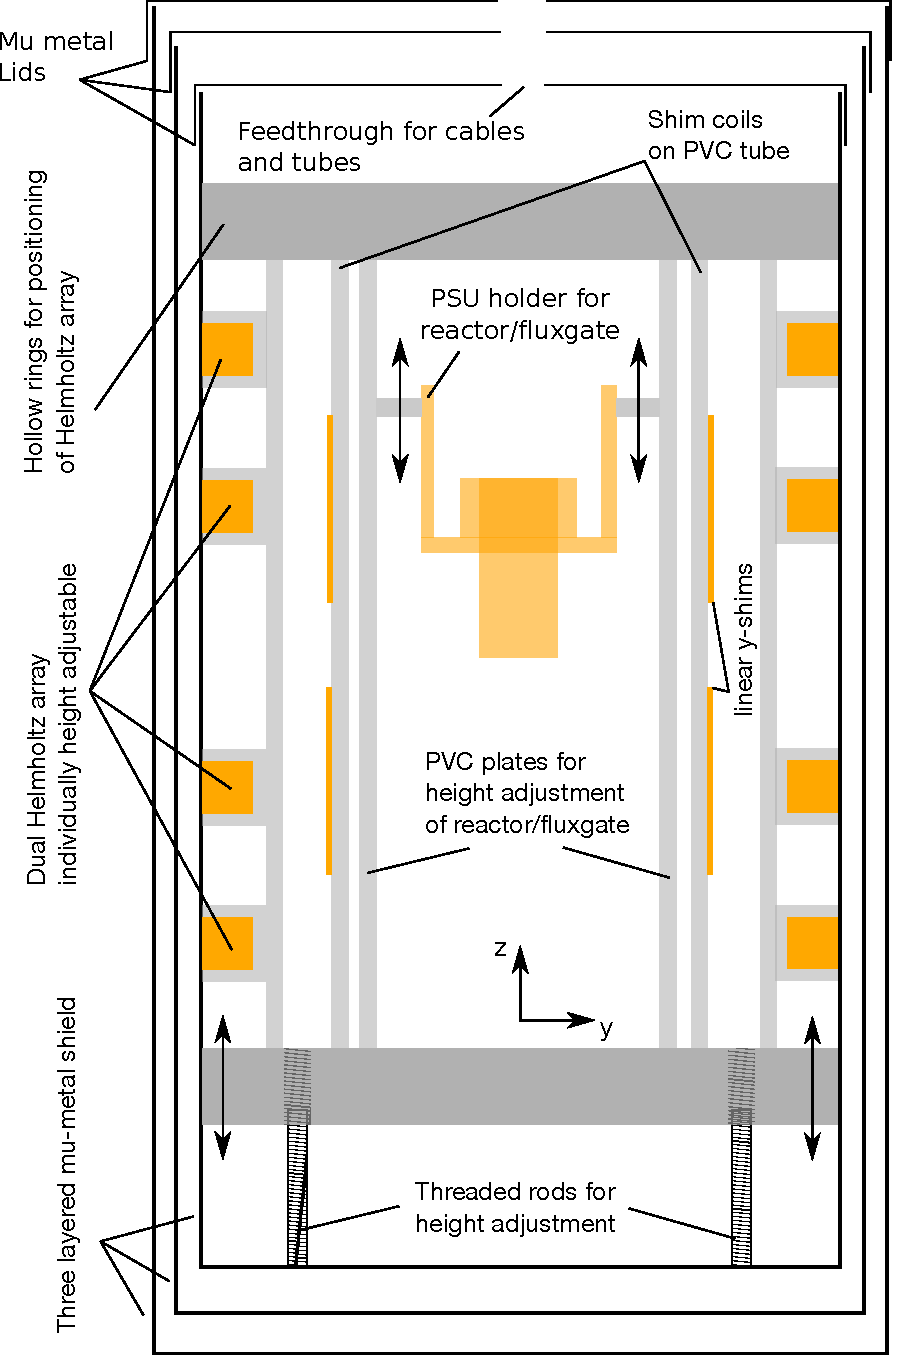
\includegraphics[width=0.95\textwidth]{/figures/materialsMethods/15NSetup/setupShield.pdf}
            \caption[Shuttling system shields]{The low field section of the SABRE shuttling system. The outermost layers represent the three layered mu metal shielding. Inside it, the form-fitted holes with the B0 coils wound onto them are displayed with the acrylic tube they're mounted onto. Further to the center, the optional shim tube is visible surrounding the low field reactor. All position adjustment directions are indicated by arrows.}
            \label{fig:matMeth:shields15N}
        \end{figure}
        \subsection{Magnetic shielding}
        To be able to polarize $^{15}\mathrm{N}$ using SABRE-Sheath (section \ref{sec:theory:15nSabre}) fields of the order of magnitude of $\SI{100}{\nano\tesla}$ are necessary to fulfill the coupling conditions described in the theory section. Thus, the setup needs to be shielded against Earth's magnetic field of typically \SI{50}{\micro\tesla}in the laboratory's lattitude. To do so, a three-layered Mu-Metal shield was purchased (ZG-209, Magnetic Shield Corp.) with a shielding factor of approximately 100 per layer. The dimensions of the shield are given in table \ref{table:matMeth:muMetalDims}.
            \begin{table}
                \centering
                \begin{tabular}{|c|ccc|}
                    \hline
                    shield no. & 1 & 2 & 3 \\
                    \hline
                    inner diameter &  \SI{229}{\mm}& \SI{254}{\mm}& \SI{183}{\mm}\\
                    height & \SI{686}{\mm}& \SI{705}{\mm}& \SI{720}\mm\\
                    wall thickness&\SI{1.57}{\mm}&\SI{1.57}{\mm}&\SI{1.57}{\mm}\\
                    \hline
                \end{tabular}
                \caption[Shield dimensions]{Dimensions of the three layers of the mu metal shield used in the setup. Note that the shields fit into each other with a gap of about \SI{1.5}{\cm} in between them. Shield 1 is the innermost, shield 3 the outermost shield.}
                \label{table:matMeth:muMetalDims}
            \end{table}
            The top caps overlap the main body by \SI{30}{\mm}.  Each cap features a central hole of \SI{25}{\mm} diameter as a feed-through for cables and tubing. Opening and closing of the caps has to be done one by one, minding cables and tubing fed through the central, sharp-edged hole. Spacers are welded onto the inner two shields outer walls to keep them centered inside the following shield further out. To move the setup around, the shield has been installed on a trolley together with the other components of the setup.  A degaussing coil was  added to the setup that merely consists of an insulated litz wire wound around the middle shield layer.
        \subsection{Degaussing setup}
        \label{sec:matMeth:degaussing}
        The degaussing coil was already installed, but no power supply was provided with it. The manufacturer suggested a current of \SI{7}{\ampere} at \SI{50}{\hertz} to be ramped down at \SI{0.25}{\ampere\per\second}. In lieu of a better alternative, a simple switch to kill an AC mains line connected to the coil was used. Both for reasons of lacking reproducibility and security reasons, this was exchanged for a current controlled, but hand-actuated power supply first and by a more sophisticated setup built by the electronics workshop later. The latter uses pulse width modulation on power MOSFETs to control the currents flowing through the coil and thus needs to be calibrated for every shield specifically. As an amperemeter is included, the calibration can be run automatically and is stored on the microcontroller. The system is controlled and calibrated by a \SI{1.6}{''} touch display. It has been precalibrated for the two shields available. The connection to the coil is established with high voltage connectors as voltages to produce the highest currents reach \SI{200}{\volt}.
        \subsection{Shim coil array}
        While they were initially designed for the low field spectrometer described before (section \ref{sec:matMeth:lowFieldSpectrometer}), the shuttling system was planned and built to enable the housing of the low field shim coils as well. These shims consist of a Maxwell coil wound around an acrylic tube to generate a linear gradient in the z direction and two assemblies of four saddle coils to generate the x- and y- shims perpendicular to the acrylic tube's rotational axis in the limited space offered.
        Figure \ref{figure:matMeth:shimCoilArray} shows the currents and fields of one of the four coil assemblies. Note that the field will differ from the shown ideal as soon as we leave the central x-y plane and move in z direction. Additionally, by the bend and the limited length of the conductors, deviations from the linear behavior of the z-field and additional x- and y-fields occur.
        \begin{figure}
            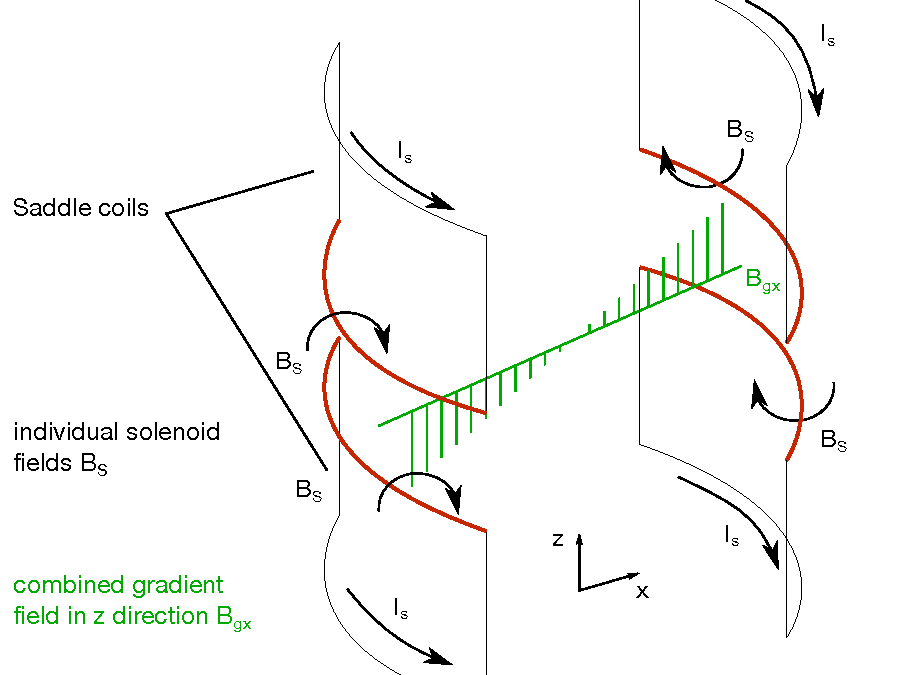
\includegraphics[width=0.99\textwidth]{/figures/materialsMethods/15NSetup/saddleCoilsShim.pdf}
            \caption[Shim coil design]{The design of the shim coils used in the setup. Note that for the x- and y- shims, a design mountable to the acrylic tube had to be used in contrast to the z-shims simple maxwell coil design. The field components $B_x$ and $B_y$ mostly cancel out in the relevant volume and $B_z$ follows a mostly linear path if the distances between the pairs are adapted to the acrylic tube's radius.}
            \label{figure:matMeth:shimCoilArray}
        \end{figure}
        \subsection{Low field reactor}
        \label{sec:matMeth:lowFieldReactor}
        At low field, multiple design features have to be combined to achieve high polarization yields.  First, pH$_2$ has to be supplied to the sample continuously and efficiently. Positioning of the probe has to be reproducible to ensure the fields are well defined.  The system must be resistant to the chemicals and solvents used in the experiments and hold the pressures applied during measurements.  Furthermore, it must be non magnetic to not distort residual fields inside the shield which otherwise might reduce polarization in parts of the sample. To fulfill all these requirements, polysulfone (PSU) was chosen as a material because of its high mechanical and chemical stability.  The reactor was designed in Inventor (Inventor 2018 Professional, Autodesk, USA) as a body of rotation. It features a sample volume of about $\SI{3}{\mm\cubed}$ with a larger diameter venting area to reduce sample losses due to foaming and spray as shown in \ref{figure:materialsMethods:probesPSU}, (a3), see indicated diameters. Below the sample volume, a interchangeable punched disk (\ref{figure:materialsMethods:probesPSU}, (a3), 2) is installed that provides pH$_2$ to the sample in fine bubbles. By changing the number and diameter of the holes, flow rate and bubble sizes can be adapted to provide pH$_2$ effectively to different kinds of samples and under different conditions. The disk can also be completely removed if only one o ring is inserted instead of the usual two. In case of sample transfer, the conical bottom collects the sample for an efficient and complete sample extraction.  Two lines connect to the bottom: one to supply pH$_2$ gas and the other to transfer the sample towards the high field.  An additional gas line connects to the top of the venting area for both de- and pressurization of the sample chamber.
        For dimensions, see appendix, section \ref{sec:appendix:reactorDims}.
            \begin{figure}
                \centering
                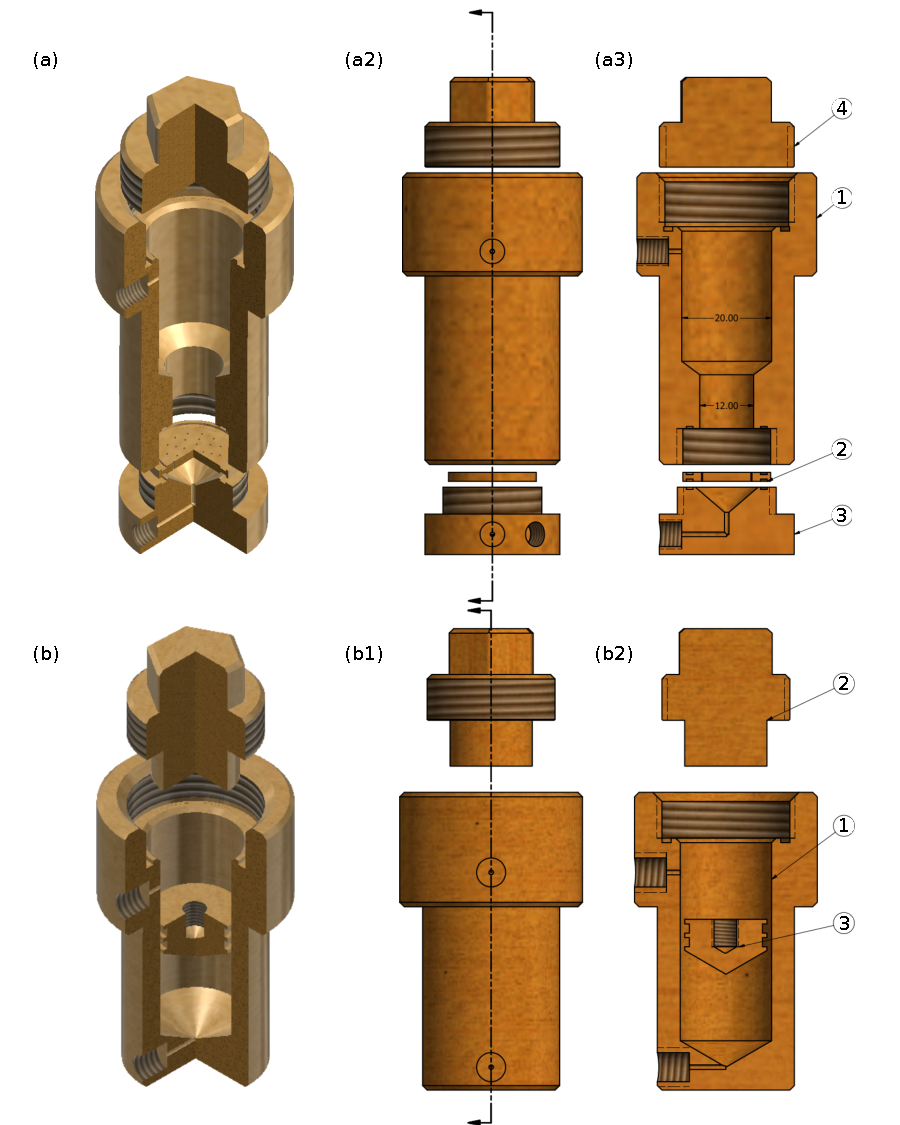
\includegraphics[width=0.99\textwidth]{/figures/materialsMethods/15NSetup/probesPSU.pdf}
                \caption[Reactor gemometry]{Three quarter section views of the low field reactor (top) and high field probe container (bottom). The disk for pH$_2$ provision in the low field reactor is visible on the bottom (a3),2 sandwiched between the main body (a3),1 and the screw on cap (a3),3.  Hose connections are made to that cap and the top of the main body. The high field probe (b2),1 is shown with its optional piston inserted (b2),3, the two possible connections at the top for actuation and bottom for sample transfer are visible in the cut views. Both pressure containers are screwed shut wit a lid (a3), 4 and (b3), 2. Seal rings are not shown here.}
                \label{figure:materialsMethods:probesPSU}
            \end{figure}
        \subsection{High field probe container}
        \label{sec:matMeth:highFieldProbe}
        Similarly to the one in low field, the high field probe has to withstand the high pressures applied and the chemicals used. It is made from the same material, PSU.  While its conical bottom is similar to the low field probe's, there's no need for a bubbling system.  Therefore, the body is made of a single part without the possibility of inserting a bubbling disk (see figure \ref{figure:materialsMethods:probesPSU}, (b2), 1).  Once the solution is transferred to the high field probe container, there are two procedures for shuttling the solution back to low field: via a piston hovering above the fluid (fig. \ref{figure:materialsMethods:probesPSU}, (b2), 3) splitting the system into a fluid and a gas side that can be actuated by pressurized gas or simply by the gas pressure that builds above the solution due to the transfer towards high field.  With methanol solutions, the latter method turns out to be efficient, other solutions with different viscosities may need the piston approach for efficient transport.
        For dimensions, see appendix \ref{sec:appendix:reactorDims}
        \subsection{Fluid handling system}
        The items described above were integrated into a fluid handling system. The whole system is connected by PTFE tubing  using ferrule connections. The tubing has \SI{1/8}{in} outer and \SI{1/16}{in} inner diameter for the gas lines and \SI{1/16}{in} outer and \SI{1/32}{in} inner diameter PTFE capillary as the fluid connection. The pH$_2$ supply line for the low field reactor is fitted with a check valve mounted as close to the reactor as possible to prohibit the sample from travelling into the supply line.
            \begin{figure}
                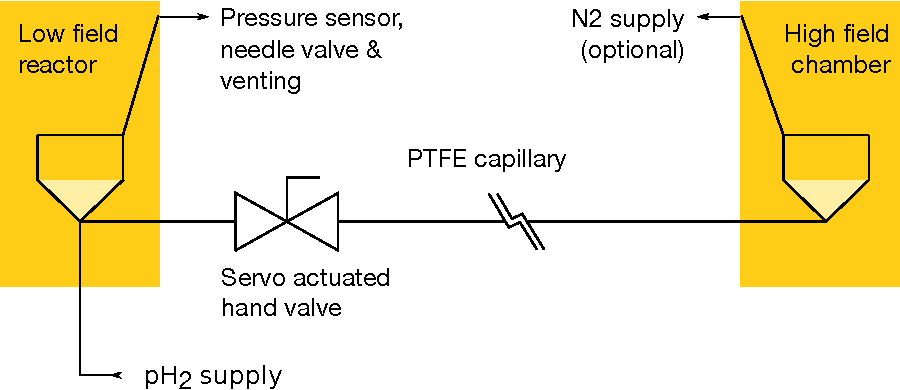
\includegraphics[width=0.99\textwidth]{/figures/materialsMethods/15NSetup/reactorsScheme.pdf}
                \caption[Reactor schematics]{The schematic of the two PTFE reactors on low field side (left) and high field side (right). The connection between both is made by a PTFE capillary separated by the automatically actuated hand valve . }
                \label{fig:matMeth:shuttlingPathway}
            \end{figure}
            Sample volumes are in the $\SI{3}{\milli\litre}$ range which means that within the rather large distances of a few meters between high and low field and reactor volumes above sample volumes to enable bubbling, close attention had to be paid to keep fluid losses as small as possible.  The choice of components therefore was focused on low volume parts.  For example, the solenoid valves used for gas supply were not an option for the fluid pathway as the internal volume was so large that different amounts of fluid remained inside the valve making reproducible measurements impossible.  The valve in the fluid transfer path was therefore chosen to be a hand valve of very small intrinsic volume ($\approx$\SI{0.05}{\ml}). The hand valve opens the same way for both sample transport directions with a different pressure gradient between high and low field side. To still be able to automate switching of the valve, a high torque servo motor (MG996R, Tower Pro) has been connected to the valve providing up to \SI{1.1}{\newton\m} torque and serving as electrically steerable actuator. That way, the fluid path consists solely of capillary of \SI{0.18}{\mm} inner diameter (\SI{1/16}{in} OD) and said hand valve. The other connections are established using \SI{1/8}{in} OD PTFE tubing.  The connections made are:
            \begin{itemize}
                \setlength{\itemsep}{-2pt}
                \item Low field chamber pressurization line
                \item Low field venting line
                \item Low field pH$_2$ supply line
                \item Needle valve outlet for bubbling
                \item Capillary connection for fluid transfer - low to high field
                \item Optional connection: high field nitrogen line for reverse transfer
            \end{itemize}
            \begin{figure}
                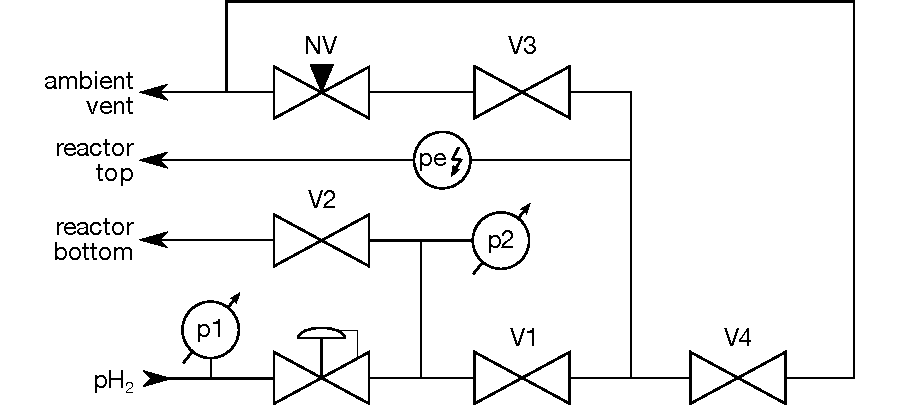
\includegraphics[width=0.99\textwidth]{/figures/materialsMethods/15NSetup/valves15N.pdf}
                \caption[Valve assembly shuttling system]{Schematic view of the valves controlled by the relay box in the shuttling setup. pH$_2$ pressure is regulated and it is distributed to the different stages of the setup. The valves labeled V1 to V6 are solenoid valves. The pressure regulator is not electronically controlled but has to be set manually. p1 and p2 are analog pressure sensors for setting up experiment pressure and monitoring bottle pressure, respectively. 'pe' is an electronic pressure sensor which's reading is fed to the microcontroller. Two additional valves (V5 and V6) to control the floating piston of the high field probe container can be added to the setup.}
                \label{fig:materialsMethods:valveSetup}
            \end{figure}
            Figure \ref{fig:materialsMethods:valveSetup} shows a schematic of the valves used in the fluid handling system. Parahydrogen supplied to the system is first pressure regulated and can then be routed to the different parts of the setup to admit pressure to the reactor from the top (V1), bubble pH$_2$ trough the solution (V2 and V3) or transfer the sample to the high field side (V1 and hand valve). The other valves are used to depressurize the reactor (V4), transfer the sample back to low field actively (V5) or passively  and vent the complete system (V1-V4). The electronic pressure sensor (indicated by the flash symbol, DRTR-AL-20MA-R60, B+B sensors) can be used to reduce pressure to a defined value on the low field side.
            A standard fluid hyperpolarization cycle would consist of: 
            \begin{itemize}
                \item Pressurization of the low field chamber to reduce initial gas flow through the sample when opening the bubbling line.  
                \item Opening the bubbling line with a certain pressure and needle valve setting for a certain time.  
                \item Closing all valves and opening the transfer line. 
                \begin{itemize}
                    \item The sample is shuttled to high field and the scanner is triggered. 
                \end{itemize}
                \item Depressurizing the low field chamber (optionally only up to a certain pressure using the pressure sensor).
                \item Reopening the transfer valve 
                \begin{itemize}
                    \item The sample flows back to low field (optionally supported by building pressure above the high field floating piston).
                \end{itemize}
            \end{itemize}
            This cycle can be repeated indefinitely, limited of course by the fluid losses through evaporation by bubbling and the spray flow towards ambient air and the overall stability of the catalyst in solution. 
            To perform these cycles in a reproducible manner, an automated system has been built controlling as much of the fluid handling system as possible.
        \subsection{Automatic shuttling system}
    To handle the probes in a reproducible manner and to produce reliable results, a system had to be designed that kept all timings and other parameters under control. A microcontroller was chosen that can be operated independent of computers or NMR/MRI machines and is quite flexible that way, i.e. can be adapted to perform different tasks. As often, the relatively cheap (~ 30 Euro) but fast (\SI{180}{\mega\hertz}) Teensy 3.6 was chosen.
            \begin{wrapfigure}{rb}{0.6\textwidth}
                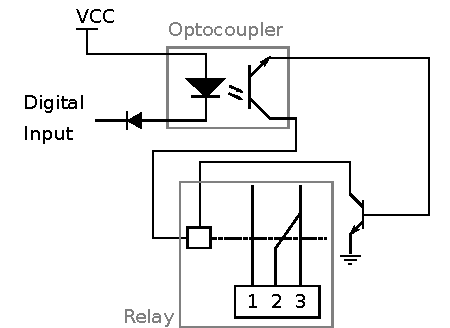
\includegraphics{/figures/materialsMethods/15NSetup/optoRelayScheme.pdf}
                \caption[Relay schematics]{One relay module of which 8 were mounted onto a single PCB board in this case. Note the galvanic isolation through the optocoupler in the top center of the schematics.}
                \label{fig:materialsMethods:relaySchematics}
            \end{wrapfigure}
            The system connects to the fluid handling system and provides it with gas pressure for fluid transport as well as gas for hyperpolarization, pH2. The system is built mostly from copper tubing (except for the low pressure vent lines). Connections are made via brass ferrule fittings and metal seals. The choice of materials provided long term stability of the system. The solenoid valves chosen were 2/2 way valves (A5241/1002/.023, GSR Ventiltechnik) of which only four were necessary for basic operation. They can handle pressures up to \SI{85}{\bar} and are operated by \SI{230}{\volt} AC. These valves were supposed to be automatically actuated.
            To do so, a relay card (Relay ISO9002, Songle Relay) was connected to all the valves to handle switching with the microcontroller. The relay can handle currents up to \SI{7}{\ampere} at voltages up to \SI{240}{\volt} AC (or \SI{10}{\ampere}, \SI{28}{\volt} DC) for resistive loads. The automation concerned the solenoid valves (that were previously actuated by flipping a switch), but also the automated hand valve and its servo motor. The microcontroller of choice was, as in many cases in this work, a Teensy 3.6 (PJRC, 3.3 V). All connections made are shown in table \ref{table:matMeth:connectionsRelaisBox}. The code operating the microcontroller can be found in the appendix. All components were installed inside a box (relay box) that featured eight female IEC sockets enabling a safe operation of the \SI{230}{\volt} valve supply voltage.  Internally, eight digital outputs of the teensy were connected to the relay card.  For galvanic isolation, a optocoupled design was chosen (see figure \ref{fig:materialsMethods:relaySchematics} for details). The workflow of the system is described in table \ref{table:matMeth:shuttlingCycle} where a activation step is followed by the hyperpolarization scheme that can be repeated over and over.
            \begin{table}
                \centering
                \begin{tabular}{|c|c|c|}
                    \hline
                    function & teensy pin & connection\\
                    \hline
                    relay switching & 25 & valve 1\\
                    of valves       & 26 & valve 2\\
                                    & 27 & valve 3\\
                                    & 28 & valve 4\\
                                    & 29 & valve 5\\
                                    & 30 & valve 6\\
                                    & 31 & valve 7\\
                                    & 32 & valve 8\\
                    \hline
                    buttons for     & 22 &button 1 \\
                    execution of                & 21 &button 2 \\
                    tasks                & 20 &button 3 \\
                                    & 19 &button 4 \\
                                    & 36 &button 5 \\
                                    & 35 &button 6 \\
                                    & 34 &button 7 \\
                                    & 33 &button 8 \\
                    \hline
                                    & 23 & servo motor \\
                    \hline
                    & 39 (A20) & pressure sensor\\
                    \hline
                                    & 0 & trigger out\\
                    \hline
                \end{tabular}
                \caption[Shuttling system pin layout]{The pins of the Teensy microcontroller used in the automatic shuttling setup. All pins are used as digital I/O pins (buttons/valves,servo,trigger) except for the pressure sensor that is a analog input.}
                \label{table:matMeth:connectionsRelaisBox}
            \end{table}
            The relay board and the teensy were supplied by a \SI{230}{\volt} AC powered \SI{5}{\volt} DC power supply.  To execute valve sequences, eight buttons were installed in the cover of the box.  Additionally, eight switches were added.  That way, depending on the program run on the teensy, switches and buttons can control either single valves directly or execute valve sequences for shuttling sample into and out of the scanner.
            \begin{table}
                \centering
                \begin{tabular}{| l | c | cccc | ccc | r |}
                    \hline
                    Step & \rotatebox{90}{Duration} & \rotatebox{90}{V1} & \rotatebox{90}{V2} & \rotatebox{90}{V3} & \rotatebox{90}{V4} & \rotatebox{90}{hand valve open} & \rotatebox{90}{scanner trigger} & \rotatebox{90}{pressure sensor} & \rotatebox{90}{comment}\\
                    \hline
                                                % 1 & 2 & 3 & 4 & HV& ST& PS& comment
                    Activation  & \SI{1}{\s}    & x & - & - & - & - & - & - & build pressure \\
                                & \SI{20}{\minute} & - & x & - & - & - & - & - & bubble for activation \\
                    \hline
\tikzmark{repBeg}    Bubbling  &\SI{20}{\s}     & - & x & - & - & x & - & - & hyperpolarize sample \\
                    \hline
                    Transfer in  &\SI{3}{\s}     & x & - & - & - & x & - & - & fluid flow \\
                                &\SI{0.5}{\s}   & - & - & - & - & - & - & - & close hand valve\\
                    \hline
                    Trigger scan&\SI{0.1}{\s}   & - & - & - & - & - & x & - & trigger module on \\
                    \hline
                  Transfer out&\SI{0.1}{\s}     & - & - & - & x & - & - & - & release pressure \tikzmark{release}\\
                            &\SI{10}{\milli\s}     & - & - & - & - & - & - & x & optional pressure read \tikzmark{pr}\\
                                &\SI{3}{\s}     & - & - & - & - & x & - & - & fluid flow \\
                    \hline
\tikzmark{repEnd}   Prepare bubbling&\SI{1}{\s} & x & - & - & - & - & - & - & build pressure again\\
                    \hline 
                \end{tabular}
                \begin{tikzpicture}[overlay, remember picture]
                    \begin{scope}[c/.style={shift={(\tabcolsep, \the\dimexpr\fontdimen12\textfont2\relax)}}]
                        \draw[->] ([c]pic cs:release) to [bend left] node[right] {feedback loop}([c]pic cs:pr);
                        \draw[->]  ([c]pic cs:pr) to [bend left]([c]pic cs:release);
                    \end{scope}
                    \begin{scope}[c/.style={shift={(-\tabcolsep, \the\dimexpr\fontdimen12\textfont2\relax)}}]
                        \draw[->] ([c]pic cs:repBeg) -- +(-.2,0) to [bend right=1] ([c, shift={(-0.2,0)}]pic cs:repEnd) -- ([c]pic cs:repEnd);
                        \draw[->] ([c]pic cs:repEnd) to [bend left=140] node[left]{$\cdot$ n}([c]pic cs:repBeg);
                    \end{scope}
                \end{tikzpicture}
                \caption[15N hyperpolarization steps]{A standard shuttling circuit as used in most of the experiments. The activation step is performed once per sample. The shuttling procedure can be repeated as often as necessary as long as the sample is still working and fluid losses are within bounds. The pressure release can optionally be performed up to a certain pressure value only.}
                \label{table:matMeth:shuttlingCycle}
            \end{table}
            In addition to the solenoid valve sockets, two low voltage parallel ports were installed.  They were used to control the servo motor of the automated hand valve and to read out the pressure sensor of the setup. More sensors or controllers can easily be added as about $\frac{3}{4}$ of the parallel port pins are still blank.
            A last outgoing connection was a coaxial jack for scanner triggering.  As described in the results section, HF-feedback from the relay made a two staged low-pass frequency filter necessary to prevent accidental scanner triggering.
    \section{Magnetic fluxgate field probe}\label{sec:methodsfluxgate}
    To measure magnetic fields very precisely, the very common hall sensor method is not sensible enough. Therefore, other principles such as squids or fluxgates have to be used at very low fields. Here, a three-axis magnetic fluxgate probe was purchased. The readout was realized using a microprocessor programmed using a USB to serial adaptor and the Arduino programming environment (Arduino 1.8.10, Arduino AG).
        \subsection{Measurement principle}
        \label{sec:matMeth:fluxgateMeasurementPrinciple}
        The measurement principle behind a fluxgate is based on the hysteresis of magnetic materials. To make use of the hysteresis effect, a ferromagnetic material is continuously polarized in alternating directions. The voltage and current throughout the hysteresis are measured. If an external field is applied to the material, this will shift the hysteresis curve as a larger field will be necessary to saturate the material in the direction countering the external field and a smaller field in the direction parallel to the external field (or its component(s)). This shift can be measured electronically and provides very precise information about the external magnetic field that causes the shift.  It can be used to measure fields in the \si{\nano\tesla} range. As the material inside the coil is not the same for all sensors and can have different defects to its structure or residual magnetization, the sensors will show offsets and need to be calibrated individually (see section \ref{sec:res:fluxgateCalibration}). This was done for 12 positions for each channel. The x- and y-channel were rotated in \SI{45}{\degree} increments while the z channel was calibrated only for a up- and a down-direction due to spatial limitations. For all positions in x- and y-direction a sine was fitted, the offset was then averaged over all positions to find the sensor offsets for x- and y-channel. Due to the limited positions in z-direction, up- and down-directions were simply averaged for each position and afterwards over all positions for the z-channel offset.
        \subsection{Power supply}
        As the fluxgate needed a power supply of $\pm$ \SI{15}{\volt} that was not provided with the sensor, a DC \SI{24}{\volt} power supply was fitted with a high efficiency $\pm$ \SI{15}{\volt} DC-DC-converter (PDM1-S24-D15, CUI INC). It features short circuit protection as well as a protection against static discharge of up to \SI{8}{\kilo\volt}. The DC-DC-converter was fitted into the power supply's casing. The original cable was replaced by a three-wire cable.
        \subsection{Arduino Uno shield}
        As a first test, a shield for a 12 bit Arduino microcontroller (Arduino Uno Rev1, BCMI, Italy) was built reading out the individual channels on individual analog inputs.  Depending on the output voltage, the signal was fed to the analog input unperturbed or split through a voltage divider if it rose above the analog inputs maximum voltage.  The shield was etched in a \SI{40}{\percent} ferric chloride solution \todo{was bei burgard dazu?} (Burgard Elektronik, Germany) bubbling bath at \SI{60}{\degree\celsius} after UV-exposure of the light sensitive PCB and development in a sodium hydroxide bath (positive developer for presensitized boards, Burgard Elektronik, Germany)  For exposure, a printed foil bag has been used into which the two sided PCB was inserted  its sides were UV-exposed individually.  As the resolution of this design was not sufficient for the low fields generated inside the mu metal shield, it had to be discarded for a solution featuring active amplification.
        \subsection{Teensy 3.6 shield}
        \label{sec:matMeth:teensyShield}
        The alternative solution to the Arduino Uno described in the previous chapter, built around a Teensy 3.6 microcontroller (PJRC, \SI{3.3}{\volt}, USA) and a self designed shield provided higher intrinsic bit depth and additional active amplification using operational amplifiers.  The board was designed using EAGLE CAD (CadSoft, USA) using the auto-routing function once the components were placed on the PCB virtually.  In most cases, the traces did not need correction, but some small details were changed e.g. to keep supply leads of the individual components short or to keep signal leads away from RF-influences.  The overall size of the board was \SI{64}{\mm} x \SI{54}{\mm}.  Top and bottom layer were connected through 66 vias, no intermediate layers were required.  The leads width was chosen to be \SI{10}{mil} (\SI{0.254}{\mm}) for both signal and power supply leads as it was deemed enough for the currents necessary. 
            Amplification was performed in two steps, all operational amplifiers were contained in a single SMD-part though (MAX44245-SO14, Maxim Integrated). Analogue switches (ADG1402, Analog Devices) were mounted for each Op-Amp, i.e. each amplification and for each channel individually. The amplifications were chosen to be 1, 4 and 16 for each of the amplification stages. The total amplification range from 1 to 256 accordingly. A precision \SI{3}{\volt} voltage reference was installed (ADR423, Analog Devices) for low noise, high precision measurements adjustable via a rotatable resistor. As a power supply, a step down (LM2675, Texas Instruments) that was fed by the $\pm$\SI{15}{\volt} dc-dc-converter of the fluxgate itself. To reduce RF-influences, a low-pass filter was fit to the data line before the analog input of the teensy. 
            \begin{figure}
                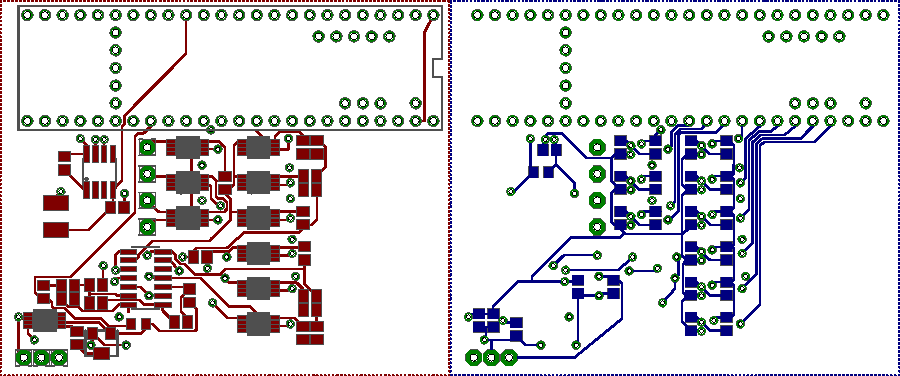
\includegraphics[width=0.99\textwidth]{/figures/materialsMethods/15NSetup/boardTopAndBottom.pdf}
                \caption[Fluxgate board layout]{The board layout of the fluxgate electronics as designed in eagle CAD. On the left, in red, the front with all the main components, i.e. ICs mounted to its surface. On the right, in blue, the back side with the supply voltage capacitors opposite of each IC. The top left three analog switches are for changing the channel, the tree next to them constitute the first amplification stage. Below is the second amplification stage that is finally read out by the teensy indicated on top.}
                \label{fig:materialsMethods:fluxgateBoard}
            \end{figure}
            \begin{table}
                \centering
                \begin{tabular}{|c|c|c|c|}
                    \hline
                    function & teensy pin & functional pin& PCB connection  \\
                    \hline
                    display&0 & sclk&\\
                    &1 & mosi&\\
                    &2 & dc&\\
                    &3 & cs&\\
                    &4 & rst&\\
                    \hline
                    channel switching&15 & & switch Z\\
                    &16 & & switch Y\\
                    &17 & & switch X\\
                    \hline
                    amplification stage 1&18 & & switch amp 1 3\\
                    &19 & & switch amp 1 2\\
                    &20 & & switch amp 1 1\\
                    \hline
                    amplification stage 2&21 & & switch amp 2 3\\
                    &22 & & switch amp 2 2\\
                    &23 & & switch amp 2 1\\
                    &A21 & & analog out\\
                    \hline
                \end{tabular}
                \caption[Fluxgate connections]{Fluxgate electronic connections as used on the final PCB.}
                \label{table:matMeth:fluxgateConnections}
            \end{table}
        \subsection{Teensy programming}
        Programs were uploaded to the microcontroller via a standard micro USB cable using the Arduino software environment. I recommend using external editors such as Vim (Vi IMproved, charityware) or Emacs (Free Software Foundation, USA) as the internal text editing functions of the Arduino environment are quite rudimentary. The program running on the teensy microcontroller reads out the three channels of the fluxgate serially with a delay of \SI{1}{\milli\second}. This delay was added to prevent switching artifacts. Each individual channel receives an amplification that is automatically adapted on the fly. Magnetic fields are calculated from the measured values using bit depth and amplification. All sensors' individual readings, the corresponding magnetic fields and the calculated total magnetic field are displayed on a simple 160x128 pixel display (1.8" mini serial SPI, IC ST7735B) driven by the Adafruit libraries (Adafruit\_ST7735.h). Note that, due to the different voltage levels of teensy and display, either a \SI{3.3}{\volt} to \SI{5}{\volt} bidirectional converter needs to be used or \SI{10}{\kilo\ohm} resistors need to be added to the data lines of the display. In addition to the final software version, several testing programs have been written: A "boardTest" program that switches the amplifications in a predefined manner to test analogue switches, a "testAmplifications" program that switches amplifications to test the analog switches and operational amplifiers and a "tftTest" program to see whether the display is connected properly and displays the expected data due to initial problems with the TFT libraries. All the testing programs use the serial I/O of the microcontroller to display data, a USB serial connection is necessary to use the full range of features.
        \subsection{Cabling and boxing}
        The complete assembly of power supply cable, teensy, display and fluxgate cable were fitted into a box with the display showing on top and connected internally \ref{table:matMeth:fluxgateConnections}. A hole for the physical USB connection to reprogram the microcontroller without opening the box was added. Note that, when plugging in the power supply, it has to be connected to the box. Otherwise, the teensy will not boot properly.
    \subsection{Error estimation}
        \subsubsection{Instrumentation}
            Statistical errors in instrumentation were estimated using the data sheets of the devices used, e.g. the microscale delivers accuracies of \SI{0.1}{\milli\gram}. A \SI{10}{\micro\liter} pipette has errors of about \SI{0.2}{\micro\liter}. Larger errors in the range of \SI{0.1}{\milli\liter} occurred when transferring larger samples and in the bubbling process through fluid loss. Additional systematic errors in instrumentation were probably present and were partly estimated.
        \subsubsection{Spectra}
        Signal area was calculated via the integral for high field spectra (linear interpolation between the points) which means the error estimation of the signal itself was done by evaluation of an equally wide integral in a noise only region of the spectrum. The absolute value of the complex spectrum in that area was used so that the maximum noise contribution (i.e. noise all in phase over the area of interest) was estimated.
            For the low field spectra, the peaks were fitted with a Lorentzian. The error of the fit concerning width and peak height were propagated for the area calculation and added to an estimation of a noise region as described for the high field spectra.
        \subsubsection{Fitting errors}
        Errors in fits were calculated using R$^2$ coefficient of determination. They were extracted from Matlab and Python fit outputs directly.
        \subsubsection{Standard deviation}
            Standard deviation of multiple measurements was calculated using
            \begin{equation}
                \sigma=\sqrt{\frac{\sum_{n=0}^N( x_n - \bar x)}{N-1}}
            \end{equation}
            where $\bar x$ is the calculated average of all measured values $x_n$.
        \subsubsection{Error propagation}
           If errors propagated in the course of an experiment, they were estimated by Gaussian error propagation, i.e. through the sum of partial deviations of the individual error sources:
           \begin{equation}
               \Delta f = \sum_{n=0}^{N}(\frac{\partial f}{\partial x_n} \Delta x_n)
           \end{equation}

% !TEX root = ../thesis_main.tex
\section{Simulation methods}\label{chapter:simulations}
\subsection{Biot Savart field simulations}
\subsubsection{$B_0$ fields in low field NMR}\label{simulations:B0}
\label{sec:simulations:B0sim}
        For $B_0$ field generation, mostly solenoid coils with compensation windings on both ends were used. To find optimal lengths and numbers of layers, Matlab simulations of static fields using Biot Savart's law were employed:
        \begin{equation}
            B(\vec r) = \frac{\mu_0}{4\pi} \int_V I\mathrm{d} \vec l \times \frac{\vec r - \vec r^{'}}{\left|\vec r - \vec r^{'}\right|^3}
        \end{equation}
        To calculate the fields, the coils were split into 30 parts per turn and each part was considered a straight, sufficiently short path for numerical integration. Two entangled loops were used to step through the windings and winding parts while the actual Biot Savart calculation for each part was performed in  3D-matrix notation for the volume of interest. This sped up the calculations compared to looping over both positions and coil elements. Additionally, a parallel pool (Matlab parallelization using multiple CPU cores) was added to reduce calculation time for the inner loop over the winding parts.
        All dimensions can be modified arbitrarily, but one has to keep in mind that results close to the coil elements will not be of real physical meaning. Nevertheless, they usually indicate well where in the graph coil elements are situated.  Both solenoidal "corkscrew" structures and closed loops were implemented and can be chosen. The measure considered for field homogeneity simulations was absolute field distribution inside a volume of $(\SI{3}{\centi\meter})^3$. Fields were calculated in a grid of $(30)^3$ points. Absolute field variation inside the volume was considered first to find the approximate range in which homogeneity is high. It was then refined by a histogram evaluation which yields results similar to the Lorentzian distribution of a Fourier transformed NMR signal. To estimate linewidths generated by field inhomogeneities, a conservative measure of the central 80 \% of field points (i.e. the central 80 \% of bins) was used to estimate the homogeneity inside the region of interest.  Using this representation and varying different parameters such as diameter, distances and relative currents in different loop structures, optimal geometries for different coil designs were calculated.
        \subsubsection{Solenoid Coil}
        The field of an infinitely long solenoid would be almost perfectly homogeneous on and along its symmetry axis. Due to the limited length of the actual coil, even on the symmetry axis, the field diverges toward the ends of the coil. Coils of finite length have been simulated using different numbers of layers and different geometric parameters. Parameters were varied in the ranges shown in table \ref{table:simulations:solenoidParameters}
        \begin{table} 
            \centering
            \begin{tabular}{|c|c|c|c|}
                \hline
                length / mm & radius / mm & wire thickness / mm & number of layers \\
                250 - 300 & 50 - 70 & 0.1 - 1.5 & 1 - 3\\
                \hline
            \end{tabular}
            \caption[Solenoid limits]{Simulation limits for the compensation windings and B0 solenoid simulation}
            \label{table:simulations:solenoidParameters}
        \end{table}
        For a schematic drawing of the coil (including compensation windings described in the next section) see chapter \ref{fig:matMeth:b0Solenoid}.

        \subsubsection{Additional Compensation Windings}
        Additional compensation windings further homogenized the field by adding a differently shaped field component that can be used to partly compensate the solenoids inhomogeneities (See figure \ref{fig:results:solenoidField} in the results section which shows the fields of solenoid and compensation windings in the x-z-plane and the resulting superposition.)
        To evaluate the field in the 3D sample volume, histograms of the field distribution were generated for different compensation wind lengths. They were used as a conservative measure of field homogeneity displaying the maximum and minimum magnetic field in the sample volume.
        \subsubsection{Dual Helmholtz Array}
        \label{simulations:DualHelmholtzArray}
        As a more advanced setup that is less prone to manufacturing errors due to the relatively larger distances to the sample volume, less error propagation during winding and a more flexible design, a dual Helmholtz array design was considered. A single Helmholtz array provides less homogeneity than a solenoid \cite{bienkowski_techniczne_2015}, but the additional pair of coils generates a differently shaped field similar to the compensation windings for the solenoid. By variation of the distances of both pairs relative to the center and their respective field strengths, i.e. the currents of the coil pairs, optimal parameters were extracted from the simulations. As the maximum and minimum radii were given by the space between mu metal shield and the shimming tube between which the B0 coil should be positioned, the variation in radius was not considered. Instead, coils were predetermined to be of inner radius \SI{125}{\mm} with twelve layers width and eight layers height per coil element.
        Additionally, absolute field values were calculated to estimate the currents necessary for $^{1}$H SABRE (i.e. to generate approximately \SI{5}{\milli\tesla}).
    \subsection{LTSpice electronics simulations}
        For designing coils and resonant circuits, simulations of the circuits makes sense to double check circuits for design errors or flaws. In cases of single resonant coils, this was not necessary due to their low complexity, but for the design of dual resonant coils, this is already useful. Electric elements can be described in detail with this software as blind inductances and capacitances can be added to the parts as well as ohmic resistances for parts that ideally would be of solely complex impedance, i.e. even complex equivalent circuits can be added as one part.
        A design is first drawn, values are then added on a part by part basis and the program can then run different analyses of the circuit. This includes AC analyses as well as DC calculations. Different step sizes can be used and different frequencies can be sampled. The flexibility is high as the input - while featuring a GUI - is actually pseudo-command line based. Circuits such as the first Arduino shield for the fluxgate were simulated to ensure proper readout of voltages. For the dual resonant, single channel circuits, different designs have been tested to find optimally performing compositions.
    \subsection{Autodesk Inventor simulations}
    The simulation toolbox of Autodesk Inventor was used to check pressure resistances of designed parts before manufacture. The program is easy to use - definitions of the materials used and the volume encased were necessary, the former is given in table \ref{table:sim:PSU} for PSU and PVC, the two materials mainly used in this work and was taken from \cite{noauthor_basf_nodate}. The parameters lower bounds were entered for all strengths to ensure that in worst case scenarios, the parts would still hold up to the stress. With the parameters entered and a closed surface defined, Autodesk uses a finite elements method to calculate the strain on the components. Display of the results is in color, but actual deformation is displayed strongly exaggerated for better visualization of the deformation that is usually small compared to the dimensions of the parts. Simulations were performed at pressures of \SI{200}{\bar} to ensure at \SI{50}{\bar}, where the maximum system pressure was supposed to be, a safety factor of 4 would be kept.
        \begin{table}
            \centering
            \begin{tabular}{|r|c|c|}
                \hline
                parameter & unit & value\\
                \hline
                thermal conductivity & $\frac{\si{\watt}}{\si{\meter} \si{\kelvin}}$ & 0.211 \\
                specific heat & $\frac{J}{g\cdot K }$ & 2.859\\
                thermal expansion coefficient & $\frac{\si{\micro\meter}}{\si{\m}\si{\kelvin}}$ & 150 \\
                Young's modulus & MPa & 911\\
                Poisson's ratio && 0.93\\
                tensile strength & MPa & 13.78\\
                yield strength & MPa & 20.67\\
                density &$(\si{\g}/\si{\cm\cubed}$) & 1.24 \\
                \hline
            \end{tabular}
            \caption[PSU properties]{The properties of PSU as used in the strain simulations in Autodesk Inventor.}
            \label{table:sim:PSU}
        \end{table}
    \subsection{Simulations using the group's spin dynamics framework}
    To estimate the field and contact times necessary for the SABRE experiments with nicotinamide, calculations previously performed in this group for pyridine \cite{knecht_spin_2014} were repeated for nicotinamide. The coupling of the sample molecule to the pH$_2$ via the catalyst was kept \cite{green_theory_2012-1} while the chemical shifts inside the molecule and thus the coupling between the internal spins were changed. Parameters are listed in table \ref{table:simulations:spinFrameworkParameters}. Indices concern the hydrogen atoms of the pairwisely added diydrogen (1,2) and the two closest hydrogen atoms on the substrate (3,4) that are coupled via the IrIMes catalyst.
        \begin{table}
        \centering
            \begin{tabular}{|c|c|}
                \hline
                parameter & value\\
                \hline
                chemical shifts & \\
                \hline
                $\delta_1$ & \SI{-22}{\hertz}\\
                $\delta_2$ & \SI{8.9}{\hertz}\\
                \hline
                J- couplings & \\
                \hline
                $J_{12}$ & \SI{7}{\hertz}\\
                $J_{13}$ & \SI{3}{\hertz}\\
                $J_{14}$ & \SI{0.1}{\hertz}\\
                $J_{23}$ & \SI{0.1}{\hertz}\\
                $J_{24}$ & \SI{0}{\hertz}\\
                $J_{34}$ & \SI{7}{\hertz}\\
                \hline
            \end{tabular}
            \caption[Spin framework parameters]{Parameters used in the spin framework simulations. Couplings between pH$_2$ and catalyst from \cite{green_theory_2012-1}. }
            \label{table:simulations:spinFrameworkParameters}
        \end{table}
